\subsection{Baseline predictions}

We began by establishing a baseline model for bass guitar tablature generation.
Initially, we utilized a pre-trained checkpoint from the DadaGP paper \cite{sarmento_dadagp_2021} without additional training.

To generate bass-specific outputs, we experimented with various prompts.
First, we provided a single bass guitar note as the initial token, however the model quickly incorporated tokens from other instruments.
This is an issue documented in the GuitarCTRL paper\cite{sarmento_gtr-ctrl_2023} where they used a metric called the UIP score (Unpromped Instrument Presence) to evaluate the model's ability to generate a specific combinations of instruments.
To constrain the output to bass tokens, we modified the logits of non-bass instruments by setting them to $-\infty$.

% FIGURE REPETITIVE GENERATION
\begin{figure}[!ht]
    \centering
    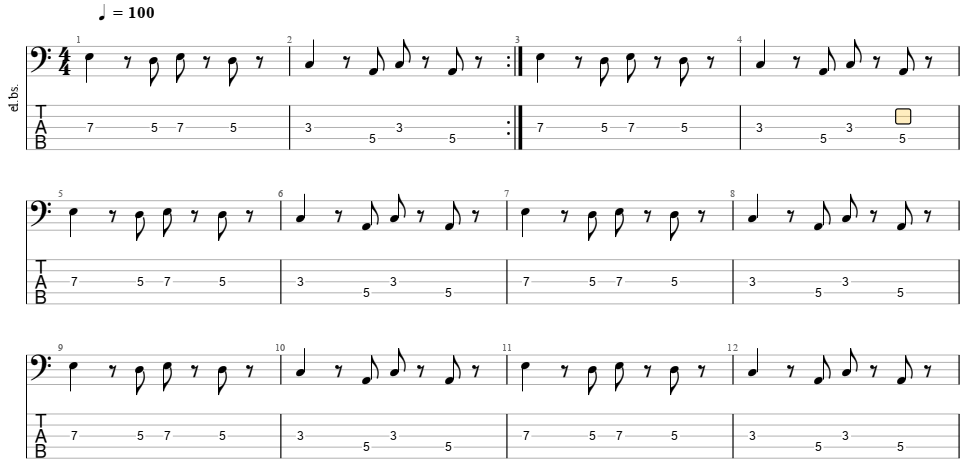
\includegraphics[width=.75\linewidth]{../images-figures/generated_bass_baseline.png}
    \caption{Example of a bass generation from the baseline model}
    \label{fig:repetitive_generation}
\end{figure}

An example of a bass tablature generated this way is shown in Figure~\ref{fig:repetitive_generation}.
While this forced the model to generate only bass tokens, the output quality was poor, featuring repetitive phrases, harmonically incorrect notes, or complete aberrations.
This was expected, as the model was not trained explicitly for bass only generation. 
Unfortunately, we cannot provide a quantitative evaluation of the generated tablatures, as we have not yet defined an evaluation metric.

\subsection{BiLSTM - Transformer model}

This section present the results we get using a model adapted from the work of Makris et al. \cite{makris_conditional_2022}.
We presented the model in section~\ref{sec:sota}.
Our data was adapted to fit the model's input requirements and the model was also slightly modified to fit our task.

% FIGURE MAKRIS ET AL. MODEL
\begin{figure}[!ht]
    \centering
    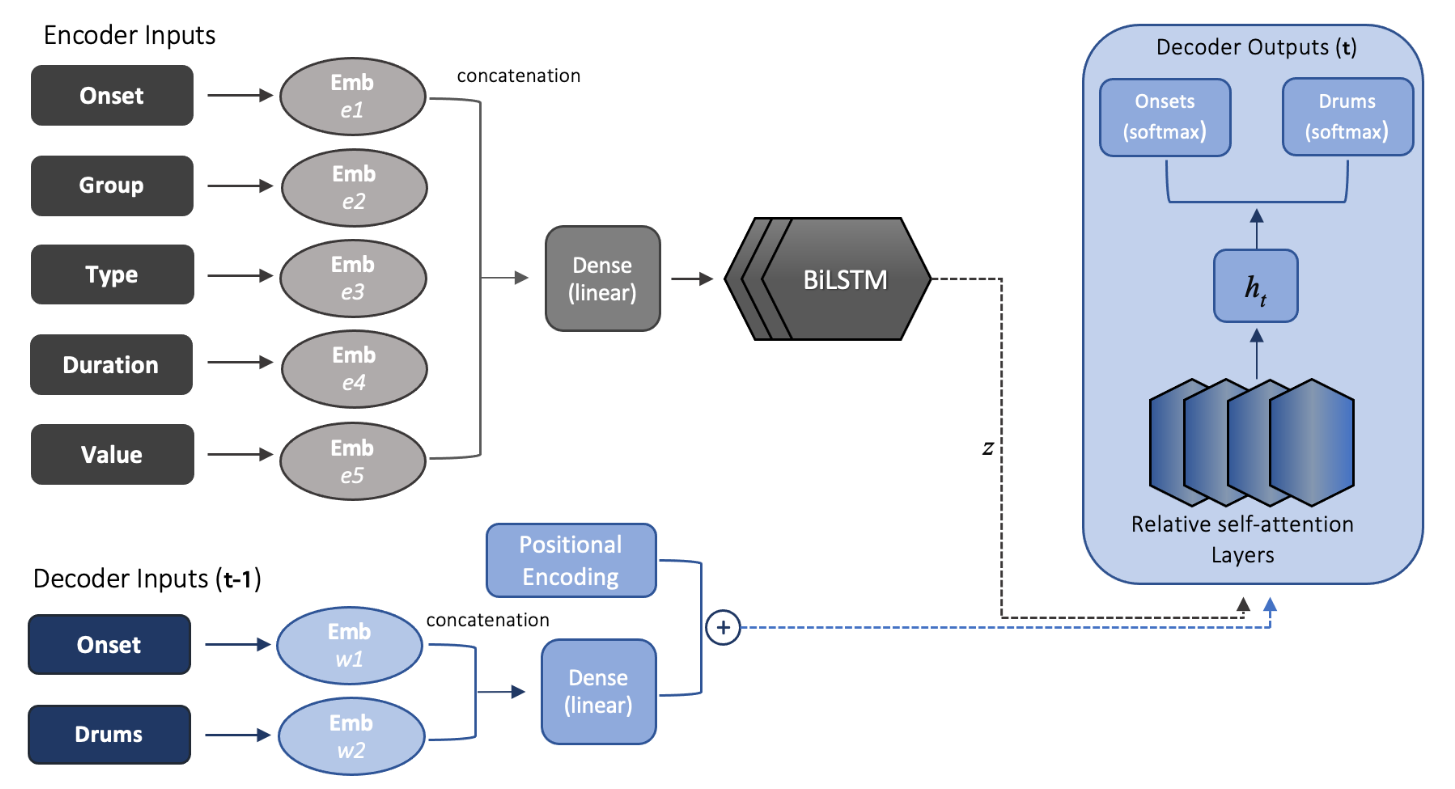
\includegraphics[width=.75\linewidth]{../images-figures/makris_model.png}
    \caption{Makris et al. model architecture, taken from their paper \cite{makris_conditional_2022}}
    \label{fig:makris_model}
\end{figure}

The figure~\ref{fig:makris_model} shows the architecture of the model proposed by Makris et al.

% FIGURE MAKRIS ET AL. MODEL ADAPTED TO OUR TASK
\begin{figure}[!ht]
    \centering
    \includegraphics[width=.75\linewidth]{../images-figures/makris_model_adapted.png}
    \caption{Makris et al. model adapted to our task}
    \label{fig:makris_model_adapted}
\end{figure}

% Workplan (what we are going to do)

% DETAILS
Our next steps include:
\begin{enumerate}
    \item Propose an evaluation metric to quantify the quality of the generated tablatures.
    \item Understand the code of the model proposed by Makris et al. using their Github repository.
    \item Adapt the model to our task and our data.
    \item Generate predictions with conditional information from several combinations of instruments.
\end{enumerate}